\documentclass[a4paper, 12pt]{book}
\usepackage[a4paper, left=0.5in, right=0.5in, top=0.8in, bottom=0.8in]{geometry}

\usepackage{hyperref} % this generates the bookmarks for PDFs
\usepackage[english]{babel}
\usepackage{amsfonts} % for math sets letters
\usepackage{amsmath} % for general math stuff
\usepackage{amssymb} % for general math stuff
\usepackage{blindtext} % generates filler text
\usepackage{paralist} % for the compactenum and compactlist procedures
\usepackage{tikz} % for tikz

\usetikzlibrary{quotes}

\setlength{\unitlength}{1cm}

% ====== MY MACROS

\newcommand{\TUG}{\TeX\ Users Group}
\newcommand{\kw}[2][\bfseries]{{#1#2}}
\newcommand{\im}[1]{{\(#1\)}}
\newcommand{\cm}[1]{{\[#1\]}} % remember that when you want to do center math you don't need to have \\ on EOL
\newcommand{\head}[1]{\textnormal{\textbf{#1}}}
\newtheorem{thm}{Theorem}
\newtheorem{dfn}[thm]{Definition}

% ====== MY MACROS

\title{TikZ introduction}
\author{Me}
\date{Jan 28, 2024}

\addtocontents{toc}{\protect{\pdfbookmark[0]{\contentsname}{toc}}}

\begin{document}
\maketitle
\tableofcontents
\chapter{TikZ Basics}
\section{\LaTeX\ built-in drawing functions}
\LaTeX\ has some basic drawing capabilities built-in, as:\\\\
\begin{picture}(1,1)
\put(0,0) {\circle{1}}    
\put(-0.5, 0) {\line(1,0){1}}
\put(-0.3, 0.06){text}
\end{picture}\\\\
This is not that good and there are a lot of other packages that works in a similar faction. TikZ is diffrent, because it allows you to \textit{program} graphics with code, witch provides more consistence and a more pleasant look. Here's how to do it in the TikZ way:\\\\
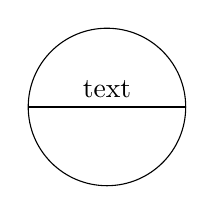
\begin{tikzpicture}
    \draw circle (1.0);
    \draw (-1,0) to ["text"] (1,0);
\end{tikzpicture}
\chapter{Creating the first TikZ images}
Lets now start to draw a \textbf{grid}.\\
\begin{tikzpicture}
    \draw[thin,dotted] (-3, -3) grid (3, 3); % from coordinate (-3,-3) to (3,3), [thin,dotted] is the option for the line
    \draw[->] (-3, 0) -- (3, 0); % draws the horizontal axis
    \draw[->] (0, -3) -- (0, 3); % draws the vertical axis
\end{tikzpicture}

\end{document}